%!TEX root = ../thesis.tex

\chapter{资料及模式介绍}

\section{原位观测}

\subsection{臭氧探空}

针对中国东南部的强对流天气,本小组成员于2019年7月25日和2020年9月1日,在南京国家基准气候站(31.93$^{\circ}$N,118.90$^{\circ}$E)共释放了五台臭氧探空仪。
为了研究对流的影响,我们分别在对流发生前和对流发生中/对流发生后各释放一次探空。
深对流概况及臭氧探空仪轨迹见图\ref{fig:ozonesonde}(a)和(b)。

\begin{figure}[!htbp]
\centering
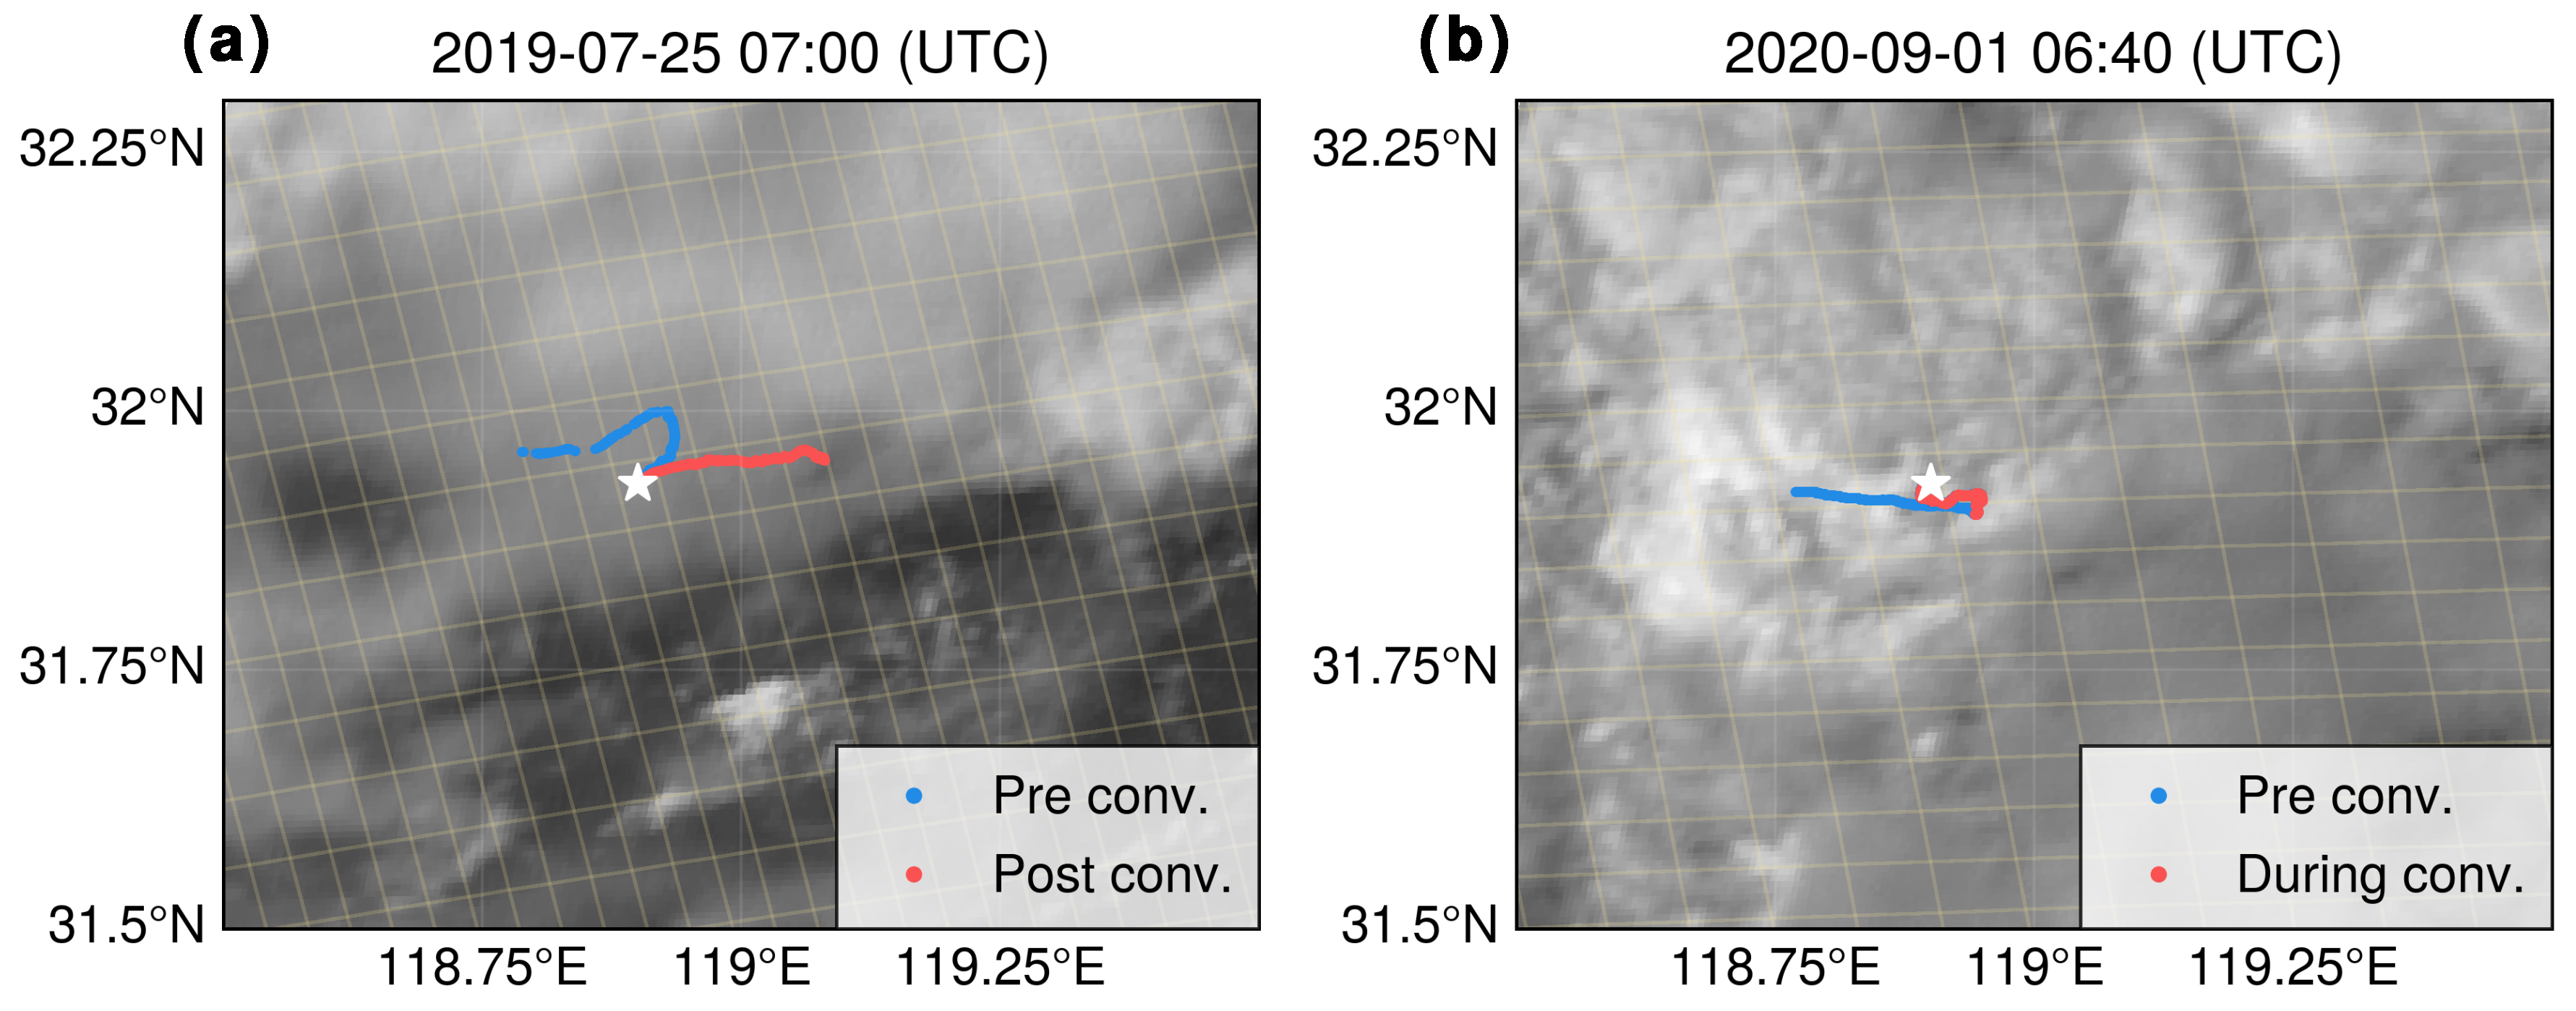
\includegraphics[width=0.9\textwidth]{./figures/ozonesonde.png}
\caption{在对流后/对流中的臭氧探空仪达到约 10 km时,风云4A先进地球静止辐射成像仪(AGRI)可见通道(0.65 $\mu$m)探测到的对流。
对流前的臭氧探空仪轨迹为为蓝色,其他为红色。白星符号代表观测站,细黄线是TROPOMI像素条带。\\
Figure \ref{fig:ozonesonde}. The convection detected by the FY-4A Advanced Geostationary Radiation Imager (AGRI)
visible channel (0.65 $\mu$m) field at the time when the post-convection/during-convection ozonesondes reached around 10 km.
The pre-convection ozonesonde trajectories are colored blue while others are in red.
The white star symbol stands for the observation station and the thin yellow lines are the TROPOMI swath pixels.
}
\label{fig:ozonesonde}
\end{figure}


具体而言,2019年7月25日发生的对流为热对流,释放的三个臭氧探空均产自中国大气物理研究所(IAP)。
IAP 臭氧探空仪使用电化学浓差电池 (ECC),其完整参数和性能见\citet{Zhang.2014}。
总体而言,从地表到2.5 km平均偏差小于0.3 mPa,9 km以下接近零,9--18 km之间小于0.5 mPa。
释放的第一台IAP臭氧探空仪于7月23日(晴天)05:35 UTC释放,另外两台分别于7月25日05:10 UTC(对流前)和06:35 UTC(对流后)释放。
由于防水故障,对流前释放的探空仪在释放后几秒钟就失去了信号,故而我们选择了7月23日释放的臭氧探空仪作为对流前的数据。
虽然时间间隔为2天,但10 km以上预报的O$_3$剖面最大相对差异通常小于25\%(图\ref{fig:waccm_forcast_o3})。
因此,臭氧日变化不足以解释探空观测到的超过65\%的差异。

此外,两台维萨拉(VAISALA)ECC臭氧探空仪分别于8月31日23:45 UTC(对流前)和9月1日06:10 UTC(对流期间)成功释放。
准备工作及具体操作均遵循标准手册,确保精度优于5\%,且在30 km 以下的精度在$\pm$ (5--10) \% 以内\citep{Smit.2007}。
该次探空试验所捕获的飑线是由冷空气和台风梅萨克(Maysak)外围环流的汇合发展而来的。
值得强调的是,对流期间的臭氧探空仪直接穿入云层,为探索受对流云影响的臭氧提供了独特的机会。



\begin{figure}[!htbp]
\centering
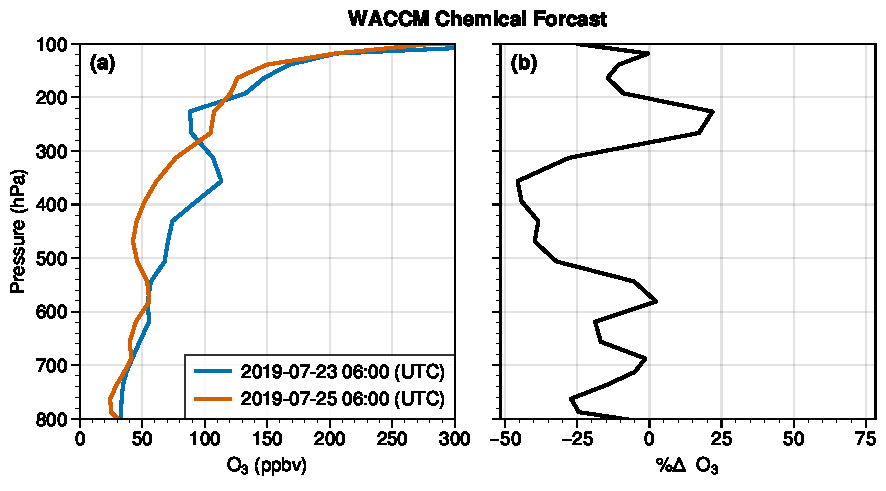
\includegraphics[width=0.9\textwidth]{./figures/waccm_forcast_o3.pdf}
\caption{(a)WACCM预测的区域平均(118.5$^{\circ}$E -- 119.5$^{\circ}$E, 31.5$^{\circ}$N – 32.5$^{\circ}$N)臭氧廓线。
蓝色为对流前,橙色为对流后。(b)为(a)中O$_3$剖面的百分比差异。\\
Figure \ref{fig:waccm_forcast_o3}. (a) Regional mean (118.5$^{\circ}$E – 119.5$^{\circ}$E, 31.5$^{\circ}$N – 32.5$^{\circ}$N)
preconvection (blue) and postconvection (orange) O$_3$ profiles from the 6-hour WACCM forecasts.
(b) The percent difference of O$_3$ profiles in (a).
}
\label{fig:waccm_forcast_o3}
\end{figure}

\subsection{闪电数据集}

在第\ref{sec:arctic}节北极的研究中,我们使用了维萨拉全球雷电数据集(GLD360)。
该闪电探测网建立于2009年,由全球极低频闪电探测传感器组成,可检测地闪和云闪\citep{Said.2010,Said.2013,Said.2017}。
地闪和云闪在北极洋面上的探测效率分别为50\%--60\% 和 < 10\%\citep{Vagasky.2022}。
因此,我们使用恒定的云闪地闪比率(约 1)来计算总闪,即修正后的总闪击为检测到的地闪闪击的四倍
\citep{Mackerras.1994,Prentice.1977}。
该常数比是根据两个要素计算的:每次闪电的闪击数(闪电多重性)和高纬度地区IC与CG闪击数的平均比(也称为Z比例)。
闪电多重性对探测效率和将闪击分组为闪电的算法较为敏感\citep{Schulz.2005,Yair.2014,Burgesser.2017,Kolmasova.2022},\citet{Yusop.2019}的高纬度研究表明闪电多重性约为1.2。
此外,高纬度闪电的平均Z比例在 1 到 1.3 之间\citep{Mackerras.1994,Prentice.1977,Bandholnopparat.2020}。
为了评估使用常数比的敏感性,我们在研究中设置了不同的值(1:2 和 2:1)来评估计算得到的LNO$_x$排放量的不确定性。


在第\ref{sec:us}节美国大陆的研究中,我们使用了整体闪电探测网(ENTLN; \citet{Marchand.2019})。
ENTLN运营着一个由全球1500多个地面站组成的系统,在美国大陆安装有900多个传感器\citep{Zhu.2017}。
云闪和地闪均由传感器根据电场脉冲极性和波形进行定位,检测频率范围为1 Hz 至 12 MHz。
如果脉冲组在700 ms和10 km范围内,则它们被归类为闪电。
在ENTLN的预处理数据中,包括了闪击和由一个或多个闪击组成的闪电。
\citet{Rudlosky.2015}将ENTLN组合事件(云闪和地闪)与闪电成像仪(LIS)测得的闪电进行了比较,
发现ENTLN在美国大陆上的闪电探测效率从2011年的62.4\%增加到2013年的79.7\%。
\citet{Lapierre.2020}还将 ENTLN 和 NLDN 数据集与2014年LIS的数据进行了比较,发现云闪闪电和闪击的探测效率分别为88\% 和 45\%。
由于我们和\citet{Lapierre.2020}一样仅使用2014年的ENTLN数据,我们采用同样的方法得到总闪的量。
具体而言,云闪闪电除以0.88,云闪闪击除以0.45,而地闪由于探测效率高,故不进行矫正。

在第\ref{sec:china}节中国东南部的研究中,我们融合了三种闪电数据集:中国国家闪电探测网(CNLDN; \citet{Yang.2015})、
ENTLN和全球闪电定位网(WWLLN;\citet{Rodger.2006})。
江苏省CNLDN数据的地闪闪电探测效率约为90\% \citep{Li.2017a},
而ENTLN和WWLLN以特定的频率(ENTLN 为 1 Hz -- 12 MHz,WWLLN 为 3--30 kHz)同时探测云闪和地闪。
WWLLN的详细处理算法由\citet{Rodger.2004}给出。
在 10 km 和 0.7 s的条件下,WWLLN测得的闪击和脉冲与ENTLN融合,构成一个数据集(ENGLN,\citet{Virts.2020b})。
为了增加我们研究中的闪电数据覆盖范围,使用 10 km 和 0.5 s 的时空聚类标准将ENGLN和CNLDN数据集的地闪数据相结合\citep{Zhao.2020},合并后的数据集应具有足够高的地闪探测效率。
由于该三种闪电数据在中国范围内的云闪探测效率较低,我们保守地使用恒定的云闪与地闪比率(3:1,\citet{Wu.2016,Bandholnopparat.2020})来得到总闪数据。
若将来有更多的中国闪电网(如北京闪电网络(BLNET;\citet{Srivastava.2017})可用于与闪电成像传感器进行比较\citep{Rudlosky.2013,Poelman.2020},云闪数据将更加准确。

\section{卫星观测}

\subsection{臭氧监测仪(OMI)}

臭氧监测仪(OMI)搭载在Aura卫星(2004年发射)上,该卫星是下午列车(A-train)卫星组的成员\citep{Levelt.2006,Levelt.2018}。
OMI在当地时$\sim$13:45(升交点)经过赤道,在 705 公里的高度以 98.2$^{\circ}$ 的倾角运行,幅宽为2600 km,最高分辨率为13 km $\times$ 24 km。
OMI是一种紫外/可见光光谱仪,光谱范围在270 nm--500 nm,光谱分辨率约为0.5 nm,可用来观测NO$_2$、SO$_2$、HCHO、BrO 和 OClO等痕量气体。
OMI 使用二维探测器,其中在探测器的一个轴上对跨轨道地面像素进行成像,在另一个轴上记录光谱信息。 这种传感技术允许同时测量条带中的所有地面像素,因此,OMI 没有扫描镜,且该二维检测器可实现宽幅、良好空间分辨率和高信噪比的组合。
OMI采用差分光学吸收光谱(DOAS)拟合来确定NO$_2$和O$_3$的垂直柱浓度,其中NO$_2$数据通常用于研究城市空气污染,评估NO$_x$排放源的影响,监测NO$_2$污染物的变化趋势等。
OMI的观测数据可以与其他大气环境监测仪器数据相结合,共同为研究者提供更全面的大气环境数据。

然而自2007年初以来,由于被称为“行异常”的异常辐射\citep{Dobber.2008},一些测量数据变得无效。
对于当前的研究,我们使用NASA标准产品v3.0\citep{Krotkov.2017}作为LNO$_x$反演算法的输入。

对流层NO$_2$垂直柱浓度($V_{\ch{LNO2}}$)的计算主要包括以下步骤。

\begin{enumerate}[label=(\arabic*), labelindent=\parindent, leftmargin=0pt, widest=0, itemindent=*, topsep=0pt, partopsep=0pt, parsep=0pt]

\item NO$_2$总斜柱浓度由 OMI 优化的差分光学吸收光谱(DOAS)拟合确定。

\item 通过从测量的总斜柱浓度中减去由仪器引起的跨道偏差,得到校正(“去条纹”)的总斜柱浓度。

\item 平流层或对流层的大气质量因子($AMF_{\ch{strat}}$,$AMF_{\ch{trop}}$)是由考虑加权散射权重的NO$_2$先验廓线的垂直积分计算得到。
这些先验廓线是GMI模式模拟的月平均先验廓线(2004--2007 年)。

\item 平流层NO$_2$垂直柱浓度($V_{\ch{strat}}$)是通过减去对流层NO$_2$的先验贡献和三步(插值、过滤和平滑)算法计算得出\citep{Bucsela.2013}。

\item $V_{\ch{strat}}$ 使用 $AMF_{\ch{strat}}$ 转换为斜柱浓度,并从测量的总斜柱浓度中减去,从而得到对流层NO$_2$斜柱浓度($S_{\ch{NO2}}$),进而 $V_{\ch{NO2}}$ = $S_{\ch{NO2}}$/$AMF_{\ch{trop}}$。

\item 基于这种方法,我们开发了一种新的 $AMF_{\ch{LNO_x}}$,通过替换原来的步骤来获得所需的 $V_{\ch{LNO_x}}$($V_{\ch{LNO_x}}$ = $S_{\ch{NO2}}$/$AMF_{\ch{LNO_x}}$)。

\item 该算法的具体细节将在第\ref{sec:amf_definition}节中讨论.

\end{enumerate}

\subsection{对流层观测仪(TROPOMI)}

2017年10月13日,搭载对流层观测仪(TROPOMI)的哨兵5号(Sentinel-5 Precursor)卫星成功发射\citep{Veefkind.2012},同OMI一样,也于每日当地时间13:30左右穿过赤道。
TROPOMI提供在四个通道(紫外、可见光、近红外和短波红外)中测量各种痕量气体浓度,以及云和气溶胶特性。
在用于NO$_2$反演的可见光通道(400–496 nm)中,光谱分辨率和采样分别为 0.54 和 0.20 nm,信噪比约为 1500。

单个地面像素为7.2 km(截至2019年8月6日为5.6 km),沿着轨迹的积分时间为1.08 s(0.84 s),在条带中间的跨轨迹方向为 3.6 km。
轨道上有450个地面像素(行),它们的大小朝向条带边缘或多或少保持不变(最大像素宽约14km)。
扫描幅宽约为2600 km,TROPOMI每天都实现全球覆盖,除了赤道处约0.5$^{\circ}$宽度的轨道之间的窄带。
由于处理中太阳天顶角($\theta_0$ $\leq$ 88$^{\circ}$)的限制,约有15\%的地面像素未处理。

在非常明亮的辐射场景(例如高云)中,包含波段4(可见;例如用于NO$_2$反演)和波段6(近红外;例如用于云数据反演)的电荷耦合器件(CCD) 探测器可能会出现饱和效应\citep{Ludewig.2020},导致某些光谱(即波长)像素的辐射率低于预期。
在饱和度大的情况下,可能会发生电荷溢出:过量电荷从饱和的行方向流入相邻的像素,导致某些光谱像素的辐射率高于预期。
1.0.0版的1b级光谱包含饱和度标记,但不包含溢出标记;2.0.0 版开始有溢出标记\citep{Ludewig.2020}。
对于本文的研究,我们使用Sentinel-5P产品算法实验室(S5P-PAL)再处理产品(v2.3.1)。
与v1.2/v1.3版本相比,新版本的产品包含的尖峰去除功能,以更好地处理探测器的饱和效应,从而在对流产生的明亮云层上提供更有效的数据\citep{Ludewig.2020,VanGeffen.2022}。
其中具有较大检索错误(processing\_quality\_flags > 0)的像素被过滤掉。

与OMI一样,$AMF_{\ch{trop}}$取决于多个参数(太阳天顶角、观察天顶角、相对方位角、表面反照率、地表气压、云分数、云高度和先验廓线):

\begin{equation} \label{eq:AMF_NO2}
AMF_{\ch{trop}} = \frac{(1-f_r) \int_{p_{surf}}^{p_{tp}} w_{clear}(p) NO_2(p) \: dp + f_r \int_{p_{cloud}}^{p_{tp}} w_{cloudy}(p) NO_2(p) \: dp}{\int_{p_{surf}}^{p_{tp}} NO_2(p) \: dp}
\end{equation}

简而言之,分子是模拟的$S_{\ch{NO2}}$,分母是模拟的$V_{\ch{NO2}}$。
其中$p_{surf}$是表面压力,$p_{tp}$是对流层顶气压,$p_{cloud}$是云压,$f_{r}$是NO$_2$窗区中的云辐射率分数,
$w_{clear}$和$w_{cloudy}$分别是查找表中的气压相关散射权重(分别用于晴天和多云条件,\citet{Lorente.2017}),
NO$_2$(p)是示踪剂模型v5(TM5)模拟的NO$_2$垂直廓线。

云压是由477 nm附近O$_2$-O$_2$碰撞吸收带反演得到的反射率加权气压\citep{Acarreta.2004,Sneep.2008,Stammes.2008}。
故深对流云的云压位于几何云顶下方,其中几何云顶与云探测卫星(CloudSat)和中分辨率成像光谱仪(MODIS)等热红外传感器检测到的值更接近\citep{Vasilkov.2008,Joiner.2012}。
因此,OMI或TROPOMI测量的对流层NO$_2$大部分位于云内部,而不是云顶之上。
下文中,“云上”或“云下”都是相对于OMI或TROPOMI测得的云压而言。
\citet{Beirle.2009}的敏感性研究比较了云底和云顶的化学成分,发现云中大部分来自闪电的二氧化氮可以被卫星探测到。
云压的概念不仅应用于LNO$_x$的研究,还应用于计算上对流层O$_3$和NO$_x$的云切片方法\citep{Ziemke.2009,Choi.2014,Strode.2017,Ziemke.2017,Marais.2018}。


\subsection{微波临边探测器(MLS)}

微波临边探测仪 (MLS) 搭载在Aura卫星上,在当地时$\sim$13:45(升交点)经过赤道。
MLS是一种热发射微波临边探测仪,可测量中间层、平流层和对流层上层温度、臭氧和其他几种痕量气体的垂直剖面。
MLS仪器主要使用240 GHz 微波波段进行臭氧反演,在 38 个压力层上(0.0215--261 hPa)具有有效的科学数据。
这些层的垂直间距在1 hPa 以下各处约为1.3 km,在 1 hPa 以上的大多数高度约为 2.7 km。
相比之下,O$_3$反演的垂直分辨率为$\approx$3 km,从 261 hPa 向上延伸到中间层。
本研究中使用的MLS O$_3$廓线数据(5.0版本)的时间段为2019年6月至8月,为了与OMI和TROPOMI匹配,我们仅使用白天的O$_3$廓线数据。
由于本文研究对象为对流云,我们参考\citet{Livesey.2013}利用冰水含量(IWC)来获得对流云条件的有效O$_3$廓线数据。
MLS的IWC产品与O$_3$数据一样,是基于 240 GHz 光谱区域(~1.2 mm)的观测结果。
在此波长下只能观察到具有大粒径的厚云(215 hPa高度的IWC $>$ 0.6 mg m$^{-3}$,\citep{Wu.2008})。 这种云通常与深对流核有关,而不是外流或局地形成的卷云。
因此,MLS IWC在本研究中用作深对流的量度,其有效范围为 215 hPa 至 83 hPa。
IWC加权函数的分析表明,215 hPa高度IWC的垂直分辨率约为4 km\citep{Wu.2008}。
\citet{Livesey.2013}采用迭代拟合算法以去除IWC产品中的一些残余晴空信号。
具体来说,这涉及计算IWC产品的每日 10$^{\circ}$纬度分辨率纬向均值,反复剔除大于均值两个标准差的数据,
并在每次迭代中重新计算剩余总体的均值和标准差。
一旦该方法收敛(通常在5--10次迭代内),任何大于 3$\sigma$ 的 IWC值都被认为是具有统计显著性的对流云并包含在平均值中(去除了纬向平均“背景”)。
此外我们使用MLS O$_3$的数据质量标志来进一步提取有效数据:准确度 $>$ 0、状态为偶数、数据质量 $>$ 1.0以及收敛度 $<$ 1.03。


\subsection{闪电氮氧化物的计算} \label{sec:amf_definition}

基于$AMF_{\ch{trop}}$,为了得到对流层LNO$_2$或LNO$_x$的垂直柱浓度,我们只需将分母改成LNO$_2$或LNO$_x$的垂直积分即可。

\begin{equation} \label{eq:AMF_LNO2}
AMF_{\ch{LNO_2}} = \frac{(1-f_r) \int_{p_{surf}}^{p_{tp}} w_{clear}(p) NO_2(p) \: dp + f_r \int_{p_{cloud}}^{p_{tp}} w_{cloudy}(p) NO_2(p) \: dp}{\int_{p_{surf}}^{p_{tp}} LNO_2(p) \: dp}
\end{equation}

当研究区域为清洁区域,式(\ref{eq:AMF_LNO2})的分子可用LNO$_2$代替NO$_2$,即

\begin{equation} \label{eq:AMF_LNO2clean}
AMF_{\ch{LNO_2Clean}} = \frac{(1-f_r) \int_{p_{surf}}^{p_{tp}} w_{clear}(p) LNO_2(p) \: dp + f_r \int_{p_{cloud}}^{p_{tp}} w_{cloudy}(p) LNO_2(p) \: dp}{\int_{p_{surf}}^{p_{tp}} LNO_2(p) \: dp}
\end{equation}

为了与前人对比,我们定义了其他两种云上的AMF,

\begin{equation} \label{eq:AMF_NO2Vis}
AMF_{\ch{NO_2Vis}} = \frac{(1-f_r) \int_{p_{surf}}^{p_{tp}} w_{clear}(p) NO_2(p) \: dp + f_r \int_{p_{cloud}}^{p_{tp}} w_{cloudy}(p) NO_2(p) \: dp}{(1-f_g) \int_{p_{surf}}^{p_{tp}} NO_2(p) \: dp + f_g \int_{p_{cloud}}^{p_{tp}} NO_2(p) \: dp}
\end{equation}

\begin{equation} \label{eq:AMF_LNO2Vis}
AMF_{\ch{LNO_2Vis}} = \frac{(1-f_r) \int_{p_{surf}}^{p_{tp}} w_{clear}(p) NO_2(p) \: dp + f_r \int_{p_{cloud}}^{p_{tp}} w_{cloudy}(p) NO_2(p) \: dp}{(1-f_g) \int_{p_{surf}}^{p_{tp}} LNO_2(p) \: dp + f_g \int_{p_{cloud}}^{p_{tp}} LNO_2(p) \: dp}
\end{equation}

其中$f_g$为云几何分数。以上各式中的NO$_2$和LNO$_2$廓线均来自于WRF-Chem的模拟结果。
由于北极地区排放源及对流模拟结果不确定性较大,本文利用基于云压假设的高斯分布来代替廓线。
高斯分布的峰宽设置为180 hPa,峰位为最高(数值最低)的OMI/TROPOMI云压。
北极地区对流云的云压范围为130$\sim$987 hPa,主要集中于250--300 hPa最常见的值(图\ref{fig:pcld_ptropo})。
由于云内部的NO$_2$浓度高,而云层之上的NO$_2$由于光解作用而浓度低,故假设的LNO$_2$廓线更加现实\citep{Beirle.2009}。
对于高而厚的云层,云层上方的散射权重相当均匀,LNO$_2$的灵敏度在云层中部附近最高,所以受LNO$_2$廓线假设的影响已降到最低\citep{Laughner.2017}。

\begin{figure}[!htbp]
\centering
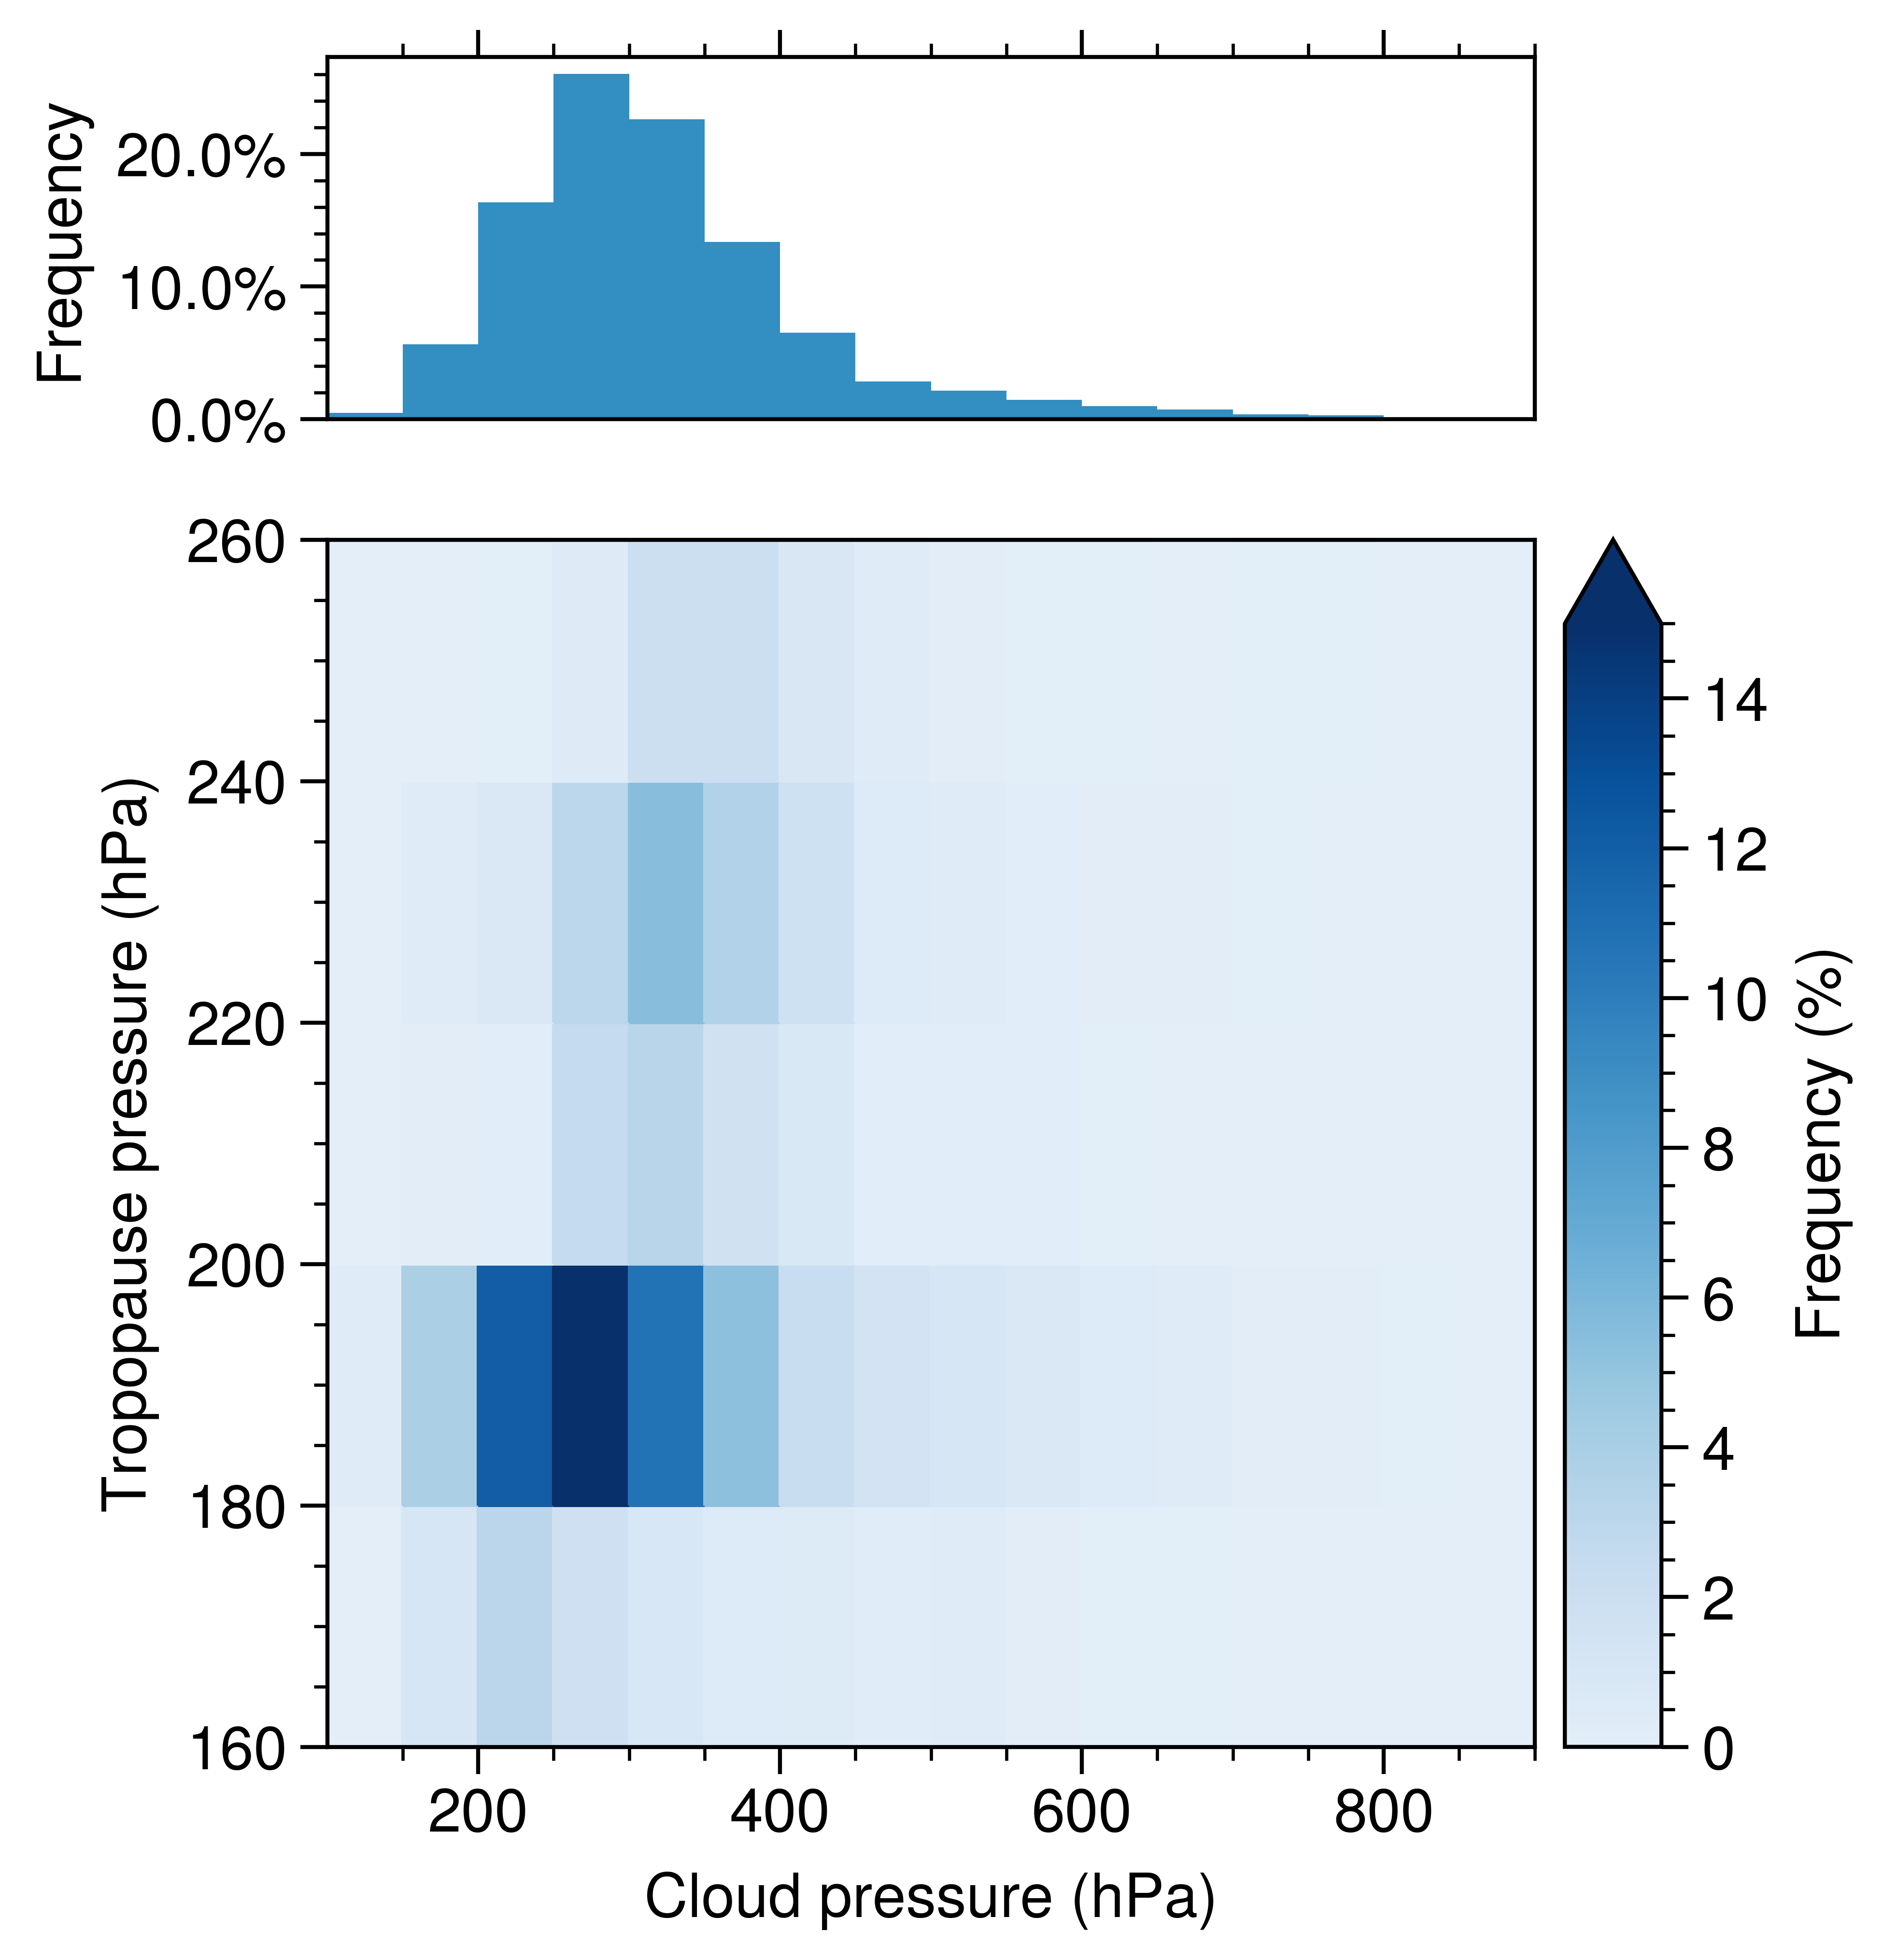
\includegraphics[width=0.5\textwidth]{./figures/pcld_ptropo.png}
\caption{云辐射分数大于0.7的像素上TROPOMI测得的云压和对流层顶高度直方图。\\
Figure \ref{fig:pcld_ptropo}. The histogram of TROPOMI cloud pressure and tropopause pressure over lightning
pixels with the cloud radiance fraction larger than 0.7.
}
\label{fig:pcld_ptropo}
\end{figure}

\subsection{云切片算法} \label{sec:cloud-slicing}

前人研究表明,云切片方法(cloud-slicing)可用于计算云内的O$_3$和NO$_2$的浓度,
该方法是计算O$_3$总柱浓度的对流云微分法(CCD)的拓展\citep{Ziemke.1998,Ziemke.2001}。
简要来说,是通过线性拟合OMI或TROPOMI测得的云上NO$_2$或O$_3$柱浓度和云压($p_{cloud}$)的斜率,从而得到NO$_2$或O$_3$的浓度,计算方法的框架见图\ref{fig:cloud-slicing_schematic}。


\begin{figure}[!htbp]
\centering
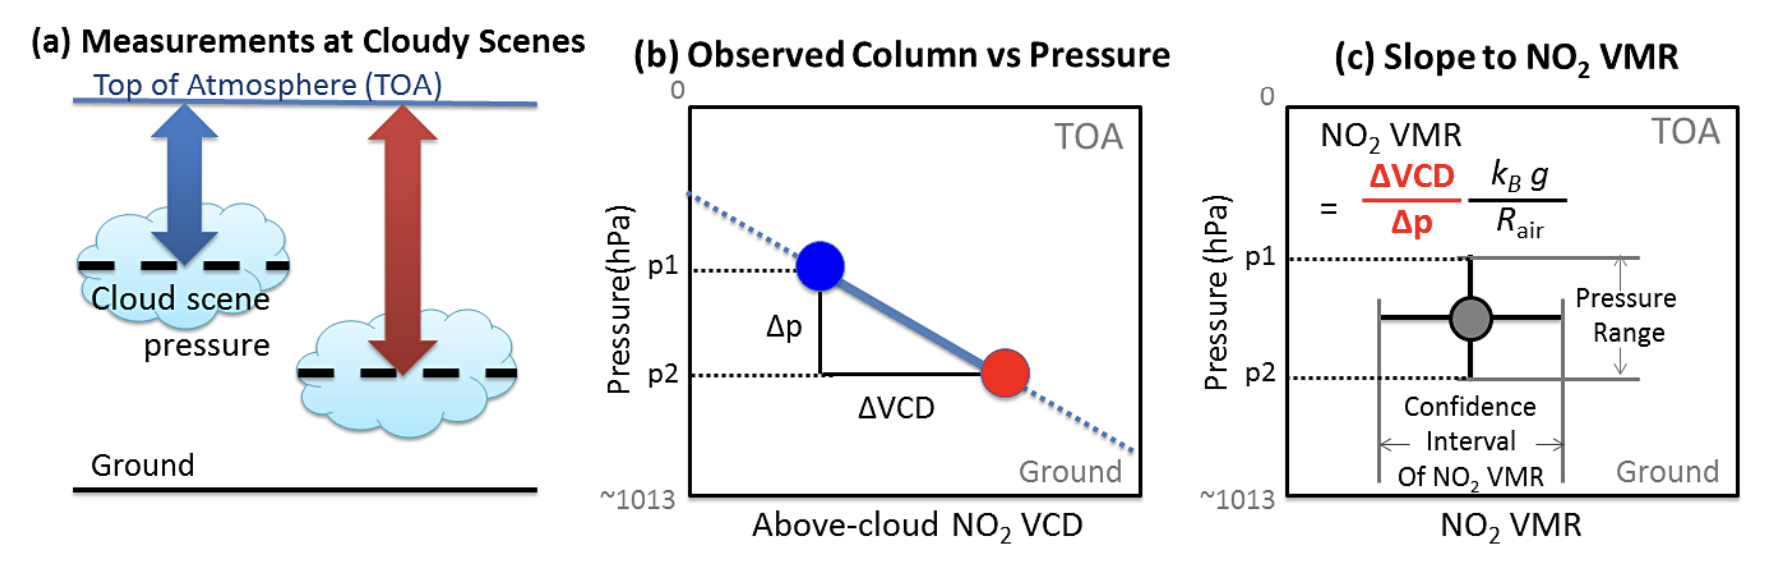
\includegraphics[width=\textwidth]{./figures/cloud-slicing_schematic.png}
\caption{云切片技术示意图(未按比例):(a) 在不同云压条件下的两次云上NO$_2$ 柱浓度测量(蓝色:云压低的柱浓度;红色:云压高的柱浓度);
(b) 在压力柱坐标平面上显示的测量值; (c) NO$_2$体积混合比(VMR)源自云上NO$_2$垂直柱浓度(VCD)与云压的斜率,置信区间为水平误差条和气压范围为垂直误差条。[图片来源:\citet{Choi.2014}]\\
Figure \ref{fig:cloud-slicing_schematic}. Schematic view of the cloud-slicing technique (not to scale):
(a) two above-cloud NO$_2$ column measurements at different cloud scene pressures (blue: column with lower scene pressure; and red: column with higher scene pressure);
(b) the measurements shown on a pressure-column coordinate plane;
(c) NO$_2$ volume mixing ratios (VMR) derived from the slope of above-cloud NO$_2$ vertical column densities (VCD) versus cloud scene pressure with confidence interval (horizontal error bar) and pressure range (vertical error bar). [Image source: \citet{Choi.2014}]
}
\label{fig:cloud-slicing_schematic}
\end{figure}

以TROPOMI的NO$_2$产品为例,对于不同的$p_{cloud}$我们需要至少两个邻近的云上$V_{\ch{NO2}}$($V_{\ch{NO2Vis}}$,图\ref{fig:cloud-slicing_schematic}a),这两个测量的结果显示在图\ref{fig:cloud-slicing_schematic}b 中的$p_{cloud}$-VCD 坐标平面中。
两个气压层$p_1$ 和 $p_2$ ($p_1$ < $p_2$) 之间的$V_{\ch{NO2}}$可以通过对$p_1$--$p_2$间的NO$_2$体积混合比 ($VMR_{\ch{NO2}}$) 进行积分得出:


\begin{equation} \label{eq:vmr_integ}
{VCD_{\ch{NO2}}}_{p_1}^{p_2}=\frac{R_{\ch{air}}}{k_Bg} \cdot \int_{p_1}^{p_2} VMR_{\ch{NO2}}(p) \mathrm{d} p
\end{equation}

其中 $R_{\ch{air}}$ 是气体常数,$k_B$ 是玻尔兹曼常数,$g$ 是重力加速度。
假设方程式\ref{eq:vmr_integ}中 $p_1$ 到 $p_2$ 范围内的混合比恒定,此气压层内的平均$VMR_{\ch{NO2}}$由下式给出:

\begin{equation}
VMR_{\ch{NO2}} = \frac{\Delta V_{\ch{NO2Vis}}}{\Delta p} \frac{k_B g}{R_{air}}
\end{equation}

从这个关系式可以看出,TROPOMI云压范围内的$VMR_{\ch{NO2}}$与$V_{\ch{NO2Vis}}$和$p_{cloud}$的拟合斜率成正比(图\ref{fig:cloud-slicing_schematic}c)。
如果有两个以上的观测值,也可以从线性拟合中推导出$VMR_{\ch{NO2}}$的置信区间,
即图\ref{fig:cloud-slicing_schematic}c中$VMR_{\ch{NO2}}$的云压范围(垂直误差条)以及置信区间(水平误差条)。
在本文中,我们利用TROPOMI、TM5、和MERRA2-GMI数据生成了各自的2019年6--8月对流层各高度区间内的平均$VMR_{\ch{NO2}}$,其中$p_{cloud}$位于以 330、450、570、670、770 和 870 hPa 为底的云压区间内。
其中由于TM5的NO$_2$为TROPOMI NO$_2$的附加产品,故利用与下文TROPOMI相同的筛选条件进行数据筛选。
而MERRA2-GMI则选择当地时下午2点的模拟数据,计算每个云层区间内的最大云量,若某区间内的最大云量$>$ 0.4,则判断该区间为多云,并计算平均$VMR_{\ch{NO2}}$。

具体而言,$V_{\ch{NO2Vis}}$有两种计算方法:
1)基于近朗伯多云AMF假设,即具有较大总光学深度的散射云均匀分布在薄层上\citep{Choi.2014};
2)几何AMF,即$AMF_{\ch{geo}}$ = sec(SZA) + sec(VZA),其中 SZA 和 VZA 分别是太阳和视角天顶角\citep{Marais.2018,Marais.2021}。
由于上对流层中NO$_2$垂直分布的不确定性\citep{Travis.2016},我们使用$AMF_{\ch{geo}}$来计算云切片方法需要的$V_{\ch{NO2Vis}}$。
\citet{Choi.2014}的研究表明,该计算方法得到的$V_{\ch{NO2Vis}}$在对流层中层(650 hPa)最多比近朗伯多云AMF方法计算的结果高14\%。
因此,$V_{\ch{NO2Vis}}$的表达式如下:

\begin{equation}
\begin{split}
V_{\ch{NO2Vis}} & = \frac{S_{\ch{NO2}}}{AMF_{\ch{geo}}} \\
             & = \frac{S_{\ch{total}}-(V_{\ch{strat}} \cdot AMF_{\ch{strat}})}{\sec (\mathrm{SZA})+\sec (\mathrm{VZA})}
\end{split}
\end{equation}

其中$S_{\ch{total}}$是总NO$_2$斜柱浓度,$V_{\ch{strat}}$为平流层NO$_2$垂直柱浓度,$AMF_{\ch{strat}}$为平流层空气质量分子。


虽然云切片方法无需知道具体的平流层NO$_2$柱浓度,即可推导出对流层的$VMR_{\ch{NO2}}$,但它依赖于以下假设和条件:
1)该方法仅适用于有相对大量的多云像素处于邻近位置,且这些像素具有足够的云压变化;
2)NO$_2$在给定的云压和空间范围内需在垂直和水平方向上充分混合;
3)平流层柱浓度在像素区域内保持不变;
4)导出的$VMR_{\ch{NO2}}$绝对量级仅与$V_{\ch{NO2Vis}}$具有一样的准确度,云压也可会带来额外的不确定性。
因此,我们参考\citet{Marais.2021}设置了以下限制条件来获得有效的云切片结果。
首先将SZA $\geq$ 80$^{\circ}$ 和表面反照率 $\geq$  30\%的像素数据去除。
接着提取多云的像素(云辐射分数[CRF] $>$ 0.7),以最大限度地减少来自下对流层的污染。
然后将每日的像素聚集到1$^{\circ}$ $\times$ 1$^{\circ}$的网格中,保留满足云压具有足够大的变化范围(云压距离 $>$ 0.5*[最高云的气压 - 最低云的气压],且标准差$>$ 30 hPa)和充分混合的NO$_2$(NO$_2$ 垂直梯度 < 0.33 pptv hPa$^{-1}$)的像素。
若网格中像素个数超过10,则将得到的$VMR_{\ch{NO2}}$赋值到该日的网格点,最后可得到各高度的季节平均$VMR_{\ch{NO2}}$。



\section{大气化学模式}

\subsection{WRF-Chem模式}

WRF-Chem是将Weather Research and Forecasting(WRF)模式与大气化学模块结合起来的大气化学模式,
可用于模拟大气中微量气体和颗粒物,研究大气动力学和化学过程之间的相互作用。
该模式包含了大量的化学反应、气溶胶过程、辐射以及各类排放源(如电力厂、交通和工业),可以准确模拟大气中各类气体和颗粒物的行为。
WRF-Chem模式的一个关键优势是它能够在高空间和时间分辨率下模拟大气化学过程,使研究人员可以详细研究地区和局部范围内化学物质和颗粒物。
此外,该模式可以采用在线和离线配置,使其成为一种灵活的工具,可以针对不同的研究问题和计算资源进行调整。
WRF-CHEM模型的另一个优势是它与其他模型(如陆地表模型和海洋模型)兼容,使研究人员可以研究土地利用、海洋和大气的相互影响和相关的化学过程。这些模型结合可以给出一个全面的地球系统研究方案。
另外,WRF-CHEM模型的数据输入和输出也很灵活,可以从大量的气象数据和大气化学数据源中获取数据,并将模拟结果输出到不同的数据格式,以方便进一步分析和研究。
总体而言,WRF-Chem具有高空间和时间分辨率、灵活性、兼容性和数据灵活性等优势,其物理和化学方案的结合使得WRF-Chem模式具有更高的科学性和实际应用价值。

WRF-Chem的物理方案包括对大气温度、压力、风速等的模拟,同时考虑了太阳辐射、长波辐射、短波辐射等因素。
同时,WRF-Chem还考虑了多种化学反应,如光化学反应、氧化反应等。
该模式的化学方案包括大气中多种物质的模拟,如空气污染物(如SO$_2$,NO$_x$等)、温室气体(如CO$_2$,CH$_4$等)、气溶胶等。
WRF-Chem的化学方案主要包括MOZCART,CBMZ和RADM2等多种方案,本研究中所使用的化学方案为MOZART(Model for Ozone and Related Chemical Tracers)。
在MOZART中,气相化学采用O$_3$和相关化学示踪剂模型版本4(MOZART4)机制\citep{Emmons.2010}。
对流层化学以81种化学物种为代表,参与38种光解和159种气相反应。
MOZART-4机制包括非甲烷挥发性有机物(NMVOC)、乙烷、丙烷、乙烯、丙烯、甲醇、异戊二烯和$\alpha$-蒎烯,
其他NMVOC物种则基于反应性官能团表示。
由于本文为了更好的模拟出深对流系统,不同的个例使用了各自的方案,具体配置见第\ref{sec:model_settings_us}节和第\ref{sec:model_settings_china}节。



\subsection{MERRA2-GMI模式}

现代研究和应用回顾分析 (MERRA-2) GMI 模拟是基于Goddard地球观测系统 (GEOS) 框架\citep{Molod.2015},使用的再分析资料为MERRA-2\citep{Gelaro.2017},化学机制为GMI(Global Modeling Initiative)的平流层和对流层化学相结合的机制\citep{Duncan.2007,Oman.2013,Nielsen.2017}。
GMI机制包括对O$_3$-NO$_x$-碳氢化合物化学的详细描述,有100多个物种和大约400个化学反应,并使用戈达德化学气溶胶辐射和传输 (GOCART) 气溶胶模块。
模拟在立方球体上运行,其水平分辨率约为 50 km,并输出到原生 MERRA-2网格(0.625$^{\circ}$ $\times$ 0.5$^{\circ}$)。

该模型以回放模式运行,\citet{Orbe.2017}对此进行了详细描述。
简而言之,该模型最初以自由状态向前运行,并与 3 小时平均MERRA2 气象场(纬向和经向风、温度、压力)进行比较。
评估两者之间的差异并倒转模型,在每个时间步长增加增量向前运行,以将模型气象学调整为 MERRA-2 再分析
评估两者之间的差异,并对模型进行倒回,以在每个时间步长上加上所需的增量,将模型气象场向MERRA-2再分析调整。
MERRA2-GMI曾用于研究对流层和平流层O$_3$,可以获得准确的O$_3$的昼夜循环、夏季臭氧与温度之间的关系以及 OMI观测到的对流层NO$_2$和O$_3$趋势\citep{Strode.2017,Ziemke.2017,Ziemke.2019}。
